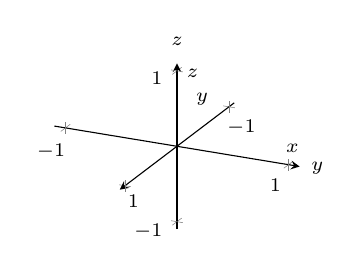
\begin{tikzpicture}
\begin{axis}%
[width=175pt,tick label style={font=\scriptsize},axis on top,
			axis lines=center,
			y dir=reverse,
			name=myplot,
			ymin=-1.1,ymax=1.1,
			xmin=-1.1,xmax=1.1,
			zmin=-1.1, zmax=1.1,
			xlabel={\scriptsize$x$},
			ylabel={\scriptsize$y$},
			zlabel={\scriptsize$z$}
]
\end{axis}
\node [right] at (myplot.right of origin)[shift={(-20pt,-8pt)}] {\scriptsize $y$};
\node [above] at (myplot.above origin) [shift={(0,-20pt)}] {\scriptsize $z$};
\end{tikzpicture}









